The total dissipation of power is composed of two major parts: dynamic and static.
The influence of process variation on the dynamic power is known to be negligibly small \cite{srivastava2010, juan2011, juan2012}; on the other hand, the variability of the static power is substantial, in which the subthreshold leakage current contributes the most \cite{juan2011, juan2012}.
Hence, we shall focus on the subthreshold leakage and, more specifically, on the effective channel length, denoted by $\Leff$, since it has the strongest influence on leakage and is severely deteriorated by process variation \cite{chandrakasan2001}.
In particular, $\Leff$ also affects other leakage-magnifying parameters such as the threshold voltage \cite{juan2011}.

It is well known that the dispersion due to process variation of the effective channel length around the nominal value resembles a bell shape, which is similar to the ones owned by Gaussian distributions.
Therefore, such variations are often conveniently modeled using Gaussian variables \cite{srivastava2010, juan2011, juan2012, chandra2010, huang2009, lee2013, shen2009, bhardwaj2006, ghanta2006}.
In this work, due to both the underlying physics and demonstration purposes, we make a step further and bake right into the model the fact that the effective channel length---occupying the space between the drain and source of a nanoscopic transistor---cannot be arbitrarily large or take a negative value, as Gaussian distributions allow it to do.
In other words, we require the model of $\Leff$ to have a bounded support.
With this in mind, we propose to model physically-bounded parameters using the four-parametric family of beta distributions: $\dBeta(a, b, c, d)$ where $a$ and $b$ are the shape parameters, and $c$ and $d$ are the left and right bounds of the support, respectively.
$a$ and $b$ can be chosen in such a way that the typically found bell shape of the distribution is preserved.
An illustration is given in \fref{beta-normal} where we fitted a beta distribution to the standard Gaussian distribution.\footnote{Alternatively, one can match the first two moments.}
It can be seen that the curves are nearly indistinguishable, but the beta one has a bounded support $[-4, 4]$, which can potentially lead to more realistic models.

\begin{figure}[t]
  \centering
  \updatedFigure{
  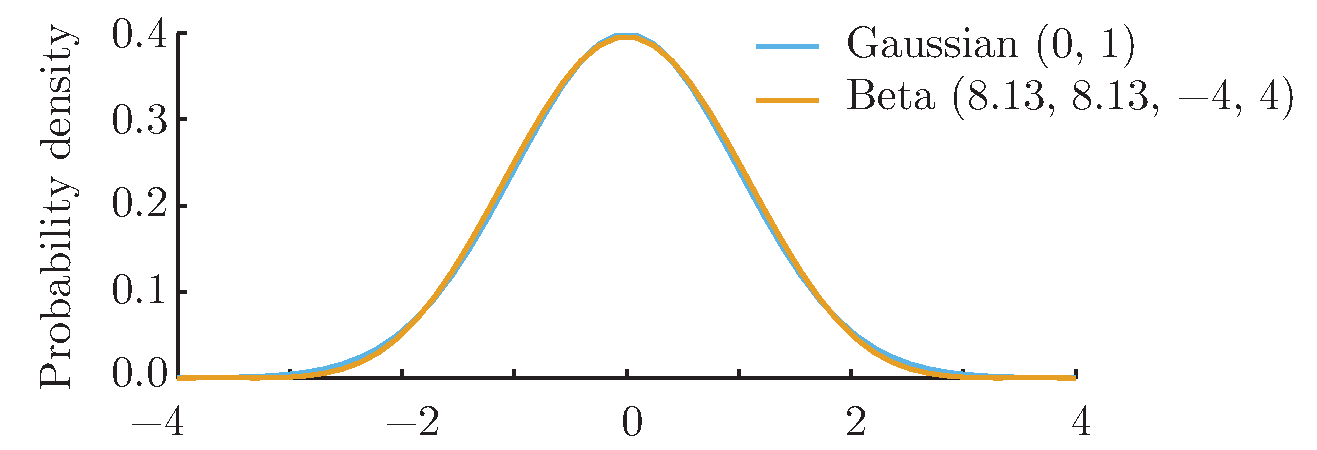
\includegraphics[width=0.9\linewidth]{include/assets/beta-normal.pdf}
  }
  \vspace{-0.5em}
  \caption{The standard Gaussian distribution and a fitted beta distribution.}
  \flabel{beta-normal}
  \vspace{-1.5em}
\end{figure}

The variability of $\Leff$ is split into global $\gLeff$ and local $\lLeff$ parts \cite{chandra2010, shen2009}.\footnote{Without loss of generality, $\gLeff$ can be treated as a composition of independent inter-lot, inter-wafer, and inter-die variations; likewise, $\lLeff$ can be treated as a composition of independent and dependent local variations.}
$\gLeff$ is assumed to be shared among all processing elements whereas each processing element has its own local parameter $\lLeff_i$.
Therefore, the effective channel length the $i$th processing element is modeled as follows:
\begin{equation} \elabel{leakage-partition}
  \Leff_i = \nLeff + \gLeff + \lLeff_i
\end{equation}
where $\nLeff$ is the nominal value of the effective channel length.
Hence, the uncertain parameters of the problem are
\begin{equation} \elabel{uncertain-parameters}
  \vU = \vec{\lLeff_1, \dotsc, \lLeff_\nprocs, \gLeff}.
\end{equation}

Global variations are typically assumed to be uncorrelated with respect to the local ones.
The latter, however, are known to have high spatial correlations, which we shall model using the following correlation function:
\begin{equation} \elabel{correlation-function}
  \oCorr{\lLeff_i, \lLeff_j} = \eta \; \fCorrSE(\vR_i, \vR_j) + (1 - \eta) \fCorrOU(\vR_i, \vR_j)
\end{equation}
where $\vR_i \in \real^2$ is the spatial location of the center of the $i$th processing element relative to the center of the die. The correlation function is a composition of two kernels:
\begin{align*}
  & \fCorrSE(\vR_i, \vR_j) = \exp\left(- \frac{\norm{\vR_i - \vR_j}^2}{\lCorrSE^2} \right) \text{ and} \\
  & \fCorrOU(\vR_i, \vR_j) = \exp\left(- \frac{\abs{\,\norm{\vR_i} - \norm{\vR_j}\,}}{\lCorrOU} \right),
\end{align*}
which are known as the squared-exponential and Ornstein-Uhlenbeck kernels, respectively.
$\eta \in [0, 1]$ is a weight coefficient balancing the kernels; $\lCorrSE$ and $\lCorrOU > 0$ are so-called length-scale parameters; and $\norm{\cdot}$ stands for the Euclidean distance.
The choice of the correlation function in \eref{correlation-function} is guided by the observations of the correlations induced by the fabrication process \cite{chandrakasan2001, friedberg2005, cheng2011}: $\fCorrSE$ imposes similarities between the spatial locations that are close to each other, and $\fCorrOU$ imposes similarities between the locations that are at the same distance from the center of the die (see also \cite{huang2009, ghanem1991, lee2013, bhardwaj2008, ghanta2006}).
The length-scale parameters $\lCorrSE$ and $\lCorrOU$ control the extend of these similarities, \ie, the range wherein the influence of one point on another is significant.

Although \eref{correlation-function} captures certain features inherent to the fabrication process, it is still an idealization.
In practice, it can be difficult to make a justifiable choice and tune such a formula, which is a prerequisite for the techniques in \sref{prior-work} based on the (continuous) KL decomposition.
A correlation matrix, on the other hand, can readily be estimated from measurements and, thus, is a more probable input to PTA.
Thus, we use \eref{correlation-function} with the only purpose of constructing a correlation matrix of $\{ \lLeff_i \}$.
For convenience, the resulting matrix is extended by one dimension to pack $\gLeff$ and $\{ \lLeff_i \}$ together.
In this case, the correlation matrix obtains one additional non-zero element on the diagonal.
Taking into account the variances of the variable, the final covariance matrix of the whole random vector $\vU$ (see \eref{uncertain-parameters}) is formed, which we denote by $\mCov_\vU$.

To conclude, an input to our analysis is the marginal distributions of the parameters $\vU$, which are beta distributions, and the corresponding covariance matrix $\mCov_\vU$.
